\section{Datenflußanalyse und \\Single-Assignment-Konversion}
%----------------------------------------------------------------------
Die Datenflußanalyse nach Feautrier \cite{Fea91} ist aufwendiger als die von
Banerjee, berücksichtigt aber auch die Optimierung.

\subsection{Ansatz}
Im Gegensatz zu Banerjee werden nicht alle Abhängigkeiten gesucht,
sondern nur echte Datenflußabhängigkeiten. Daher werden nicht alle
Zugriffspaare untersucht, sondern zu jedem Lesezugriff werden alle
Schreibzugriffe als mögliche Quellen betrachtet. Der Lesezugriff ist
damit die Senke; der Typ der Abhängigkeiten ist \emph{flow}.

Durch diesen Ansatz wird die Existenz des Lesezugriffs zu einer immer
erfüllten Voraussetzung, die für das Konfliktgleichungssystem und die
Existenz der Quelle oder auch die Optimierung zusätzliche Informationen
bedeutet.

Das System aus Konfliktgleichungen, Existenzungleichungen und
Ordnungsungleichungen wird einem Tool zur parametrisierten, ganzzahlig
linearen Optimierung (z.B. PIP) in einem Aufwasch präsentiert.

Die (lokal bereits optimierten) Lösungsergebnisse werden in einem
zweiten Arbeitsgang ``gemischt''.

Resultat: für Polyeder: eindeutige Quellen je Lesezugriff.

\subsection{Single-Assignment-Konversion}
\begin{enumerate}
\item einmalige Zuweisung durch ``Umleiten'' der Schreibzugriffe in
  neue Arrays, die voll indiziert sind.
\item Wiederherstellung der Semantik durch Einsetzen der Quelle in den
  Lesezugriffen.
\end{enumerate}

\subsection{Verfahren von Feautrier:}
Bei Feautrier ist die Ordnung das \emph{Input Kriterium}. Damit sind alle Gleichungen in ein System pro Dimension aufstellbar. (Für die Antiabhängigkeiten (wg. der Inputvernachlässigung) gibt es keine derartige Optimierung, da man nicht überlesen kann.)
\entrymodifiers={++[][]}

\xymatrix{
*+[F]{x = \dots} \ar[d] |{Datenfluss}
          \ar@/^6pc/[ddd]|{Banerjee-Abh.}\\
*+[F]{\dots = x} \ar[d] |{Anti-Abh.} \\
*+[F]{x = \dots} \ar[d] |{Datenfluss}\\
*+[F]{\dots = x}
}

~\\[0.5cm]
\emph{Konfliktgleichungssystem:} gleich Banerjee\\[0.2cm]
\emph{Existenz-Ungleichungen:} Welche \glqq Writes \grqq schreiben den an der aktuellen Stelle gelesenen Wert? Welches \glqq Write \grqq ist das letzte? $\leftarrow$ Optimierung\\[0.2cm]
\emph{Read-Existenz:} Kontext für die Analyse, Feautrier liefert nur optimierten True-Deps., also die Flow-Dependences.\\[0.2cm]
\emph{Folge:} die Ordnung wird Input des Verfahrens:\\
als Ungleichungssysteme (je Fall für die lexikographiesche Ordnung eine)

\subsubsection{Beispiel}
\textit{Programmcode:}

\begin{procedure}[H]
\SetLine
\For{$i=0$ \KwTo $n$}{
    \textbf{R:} $A[0,0] := ...$\\
    \textbf{S:} $X[i]   := A[i,0]$\\
    \For{$j=1$ \KwTo $n$}{
        \For{$k=1$ \KwTo $n$}{
            \textbf{T:} $A[i+k-1,j-1]:=...$\\
        }
    }
}
\end{procedure}

\textit{Frage:} Wer hat den Wert geschrieben, der in $\langle (i),S \rangle$ gelesen wird?\\

\textbf{S-T-Konflikt}\\
\begin{enumerate}
    \item \textit{Instanz:} $\langle (i), S \rangle$, $\langle (i^\prime, j^\prime, k^\prime), T) \rangle$

    \item \textit{Konfliktgleichungssystem:} \\
        $\begin{array}{cc}
        \left.
        \begin{array}{c@= l}
            i & i^\prime + k^\prime-1\\
            0 & j^\prime -1
        \end{array} \right\} & \Leftrightarrow
        \begin{array}{c@= l}
            k^\prime & i-i^\prime +1 \\
            j^\prime & 1
        \end{array}
        \end{array}$


    \item \textit{Existenzungleichungen:} nur für $i^\prime, j^\prime, k^\prime$\\
        \begin{align*}
        0 &\leq i^\prime \leq n \\
        1 &\leq j^\prime \leq n \\
        1 &\leq k^\prime \leq n
        \end{align*}
        Kontext: $0 \leq i \leq n$\\
        (Da hier kein Interesse für Anti-Abhängigkeiten besteht, erfolgt alles im Kontext von i. \glqq Ich bin Statement S, welche Iteration hat geschrieben, was ich gerade lese?\grqq)
    \item \textit{Ordnung:} soll $\langle ( i^\prime, j^\prime, k^\prime), T \rangle \rightarrow \langle (i), S \rangle$\\

    $(i^\prime < i) \lor \underbrace{(i^\prime = i \land \text{T textuell vor S})}_{false}$


$
\begin{array}{cc}
% \begin{array}{cc}
% \left.
\begin{array}{cccccc}
i^\prime & j^\prime & k^\prime & i & n & 1  \\
-1       & 0        & -1       & 1 & 0 & 1  \\
1        & 0        & 1        & -1& 0 & -1 \\
0        & 1        & 0        & 0 & 0 & -1 \\
0        & -1       & 0        & 0 & 0 & 1  \\
% \end{array}\right\} & Konfliktgleichungen\\
% \left.
% \begin{array}{cccccc}
1        & 0        & 0        & 0 & 0 & 0  \\
-1       & 0        & 0        & 0 & 1 & 0  \\
0        & 1        & 0        & 0 & 0 & -1 \\
0        & -1       & 0        & 0 & 1 & 0  \\
0        & 0        & 1        & 0 & 0 & -1 \\
0        & 0        & -1       & 0 & 1 & 0  \\
% \end{array} \right\} & Existenzungleichungen\\
% \left.
% \begin{array}{cccccc}
0        & 0        & 0        & 1 & 0 & 0  \\
0        & 0        & 0        &-1 & 1 & 0  \\
% \end{array} \right\} & Kontext\\
% \left.
% \begin{array}{cccccc}
-1       & 0        & 0        & 1 & 0 &-1
% \end{array} \right\} & Ordnung i^\prime < i\\
\end{array}
& \geq 0
\end{array}$\\

(Die ersten vier Zeilen sind das Konfliktgleichungssystem, dann folgen 6 Zeilen lang das Existenzungleichungssystem, dem sich dann eine Kontextzeile und eine Ordnung (\( i^\prime < i \)) anschließt.)
Lösung des Gleichungssystems mit FM.\\

Zwischenergebnis: \\$\langle (i^\prime, 1, i-i^\prime+1), T \rangle \rightarrow \langle (i), S \rangle *\\$ für $ 0 \leq i^\prime < i \leq n \text{, } 1\leq i-i^\prime + 1 \leq n \\
\text{ für Kontext } 0\leq i \leq n$

\item \textit{Optimierung}\\
    gesucht: letzte (lex. größte) Instanz von T mit *, die vor $\langle (i), S \rangle$ ausgeführt wird. \\
    Lösung: $i^\prime = i-1\\
            \Rightarrow \langle (i-1,1,2), T \rangle \rightarrow \langle (i), S \rangle$ für $i \geq 1$
\end{enumerate}

\textbf{S-R-Konflikt}\\
    \begin{enumerate}
    \item $\langle (i), S \rangle \text{,} \langle(i^\prime), R \rangle$
    \item $0=i \land 0 = 0$
    \item $0 \leq i^\prime \leq n \text{ im Kontext } 0 \leq i \leq n$
    \item $i^\prime < i \lor (i^\prime = i \land \text{ R vor S}) \Leftrightarrow i^\prime \leq i$
    \item $i^\prime = i \\
        \Rightarrow \langle (i),R \rangle \rightarrow \langle (i), S \rangle \text{ für } i=0 \\
        \Rightarrow \langle (0),R \rangle \rightarrow \langle (0), S \rangle$

    \end{enumerate}
Datenfluss: \\
\begin{procedure}
    src($ \langle (i), S \rangle $) =\\ \eIf{$i=0$}{$\langle (0), R \rangle$}{$\langle (i-1,1,2),T \rangle$}
\end{procedure}

Vorsicht: Falls die Bedingungen der Schleifenindizes nicht disjunkt sind, geht die Abhängigkeit von Maximum der Quellen (bzgl. der Ausführungsordnung) aus.

%% --------------------------- CfFada -------------------------------------------------

\subsection{Verfahren via CfFada:}

CfFada heißt ausgeschrieben \glqq Controllflow based Fuzzy array dataflow\grqq.\\
Dieses weiteres Verfahren wird motiviert durch die Existenz von \glqq if-Statements\grqq\ , \glqq unstrukturierte Programme\grqq\ und die erhöhte \glqq Präzision\grqq.\\
\paragraph{Idee:}
\begin{enumerate}
    \item Zusammenführen von
    \begin {enumerate}
        \item traditionellen (universell einsetzbar, ungenau) und
        \item einem Feautrier-ähnlichem Verfahren
    \end{enumerate}
    \item (Effizienz)
\end{enumerate}

\paragraph{Prinzipielles Vorgehen:}
\begin{enumerate}
    \item Konstruiere den Kontrollflußgraphen (CFG)
    \item Für jeden Zugriff a:
        \begin{enumerate}
            \item Annotiere den CFG mit den für a relevanten Relationen - unter Berücksichtigung der umgebenden Prädikate
            \item starte mit leerer Abhängigkeitsmenge (alles bottom) und Ordnungsrelation $(=,...,=)$ bei a. (\( i = i^\prime = \dots \))
            \item durchlaufe den CFG rückwärts
            \item bei Schleifen: durchlaufe die Rückwärtskanten von innen nach außen und passe die aktuell gültige Ordnungsrelation an
            \item bei \glqq conflicting accesses\grqq : mische die neuen und alten Abhängigkeiten unter Berücksichtigung der Optimierung
        \end{enumerate}
\end{enumerate}


\paragraph{Anmerkungen:}

\begin{enumerate}
    \item Implementierung mit Omega (Presburger Arithmetik) \( \rightarrow \) Genauigkeit
    \item unstrukturierte Programme \( \rightarrow \) Abschätzung der Ordnungsrelation
    \item vorzeitiges Analyse-Ende möglich, wenn alle möglichen letzten Quellen gefunden wurden.
    \item Der Hauptunterschied zu Feautrier besteht in der Tatsache, dass CfFada mit if-Statemants umgehen kann.
    \item textuell getragene Abhängigkeiten entspricht sprachlich den Schleifenunabhängigen Abhängigkeiten
    \item Mischen: Schneiden und Optimierung
    \item \( \Box := \) Merge/Mischen
    \item \( W(6) := \) Write-Set von 6
\end{enumerate}


\subsubsection{Beispiel zur Abhängigkeitsanalyse nach CfFada}

\begin{wrapfigure}{r}{0.6\textwidth}
    \begin{flushright}
        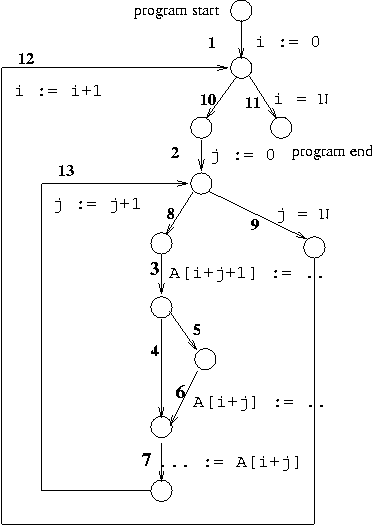
\includegraphics[scale=0.5]{images/cffada.png}
        \caption{Ablaufgraph}
        \vspace{+40pt}
    \end{flushright}

\end{wrapfigure}

\textit{Programmcode:}\\
    \begin{procedure}[H]
    \SetLine
    \For{$i=0$ \KwTo $N$}{
        \For{$j=0$ \KwTo $N$}{

            \bf{3:} $A[i+j+1]$ = ... \\
            \eIf{$P$}
                {\bf{6:} $A[i+j]$ = ...\\}{}
            \bf{7:} ... = $A[i+j]$

        }
    }
    \end{procedure}

~\\[6cm]
\textbf{Kontext}\\
Read-Statement 7\\
Operationen: $\langle (i,j), 7 \rangle$ für $0 \leq i, j \leq N$\\
\\
\textbf{Annotierung}\\
Statement 3\\
Operationen: \(\langle (i^\prime,j^\prime), 3 \rangle\) für \( \underbrace{0 \leq i^\prime, j^\prime \leq N}_{Existenz} \land \underbrace{i^\prime + j^\prime + 1 = i + j}_{Konflikt}\)\\
Statement 6\\
Operationen: \dots\\

\textbf{Durchlauf}\\
\begin{enumerate}
    \item {Ordnung: \(i=i^\prime \land j=j^\prime\) \\
        \(src^{(0)} = {\perp}\)\\
        \begin{enumerate}
            \item Start: 7
            \item die 4 hoch: (Kante mit Label 4)\\
                  Keine neuen Quellen\\
                  \(scr_{4}^{(1)} = \lbrace \perp \rbrace\)
            \item die 6 hoch: (überprüfe Existenzun- und Konfliktgleichungen)\\
                  \(src_{6}^{(1)} = src^{(0)} \Box W(6) = \)
    \(\begin{cases}  \langle (i,j), 6 \rangle , & \mbox{ für } P^\prime(i,j) \\
                     \perp ,                    & \mbox{ sonst }
    \end{cases}  \)

            \item bei n1 Mischen:\\
                \(scr_{n1}^{(1)} =
    \begin{cases} \langle (i,j),6 \rangle, & \mbox{ für } p^\prime(i,j) \\
                  \perp,                   & \mbox{ sonst }
                \end{cases} \)

            \item die 3 hoch:\\
                  Keine neuen Quellen, da die aktuelle Ordnung $\lightning$ Konfliktgleichung. (Wäre P immer true, könnte man an n1 abbrechen.)
            \item die 13 hoch \(\Rightarrow\)

        \end{enumerate}
        }
    \item {Ordnung: \(i=i^\prime \land j^\prime < j\) \\
      \begin{enumerate}
         \item die Kanten 7, 4 bringen nichts neues.
         \item die 6 hoch: \\
           Keine neuen Quellen, da die aktuelle Ordnung $\lightning$ Konfliktgleichung.
         \item n1: nichts neues zu mischen \(\Rightarrow\) alles bleibt
         \item die 3 hoch: \\
           \(src^{(2)} = src^{(1)} \Box W(3) = \) \\ \( =
           \begin{cases} \langle ( i^\prime, j^\prime), 3) \rangle, & \mbox{ für } i^\prime + j^\prime + 1 = i + j \land \neg P^\prime(i,j) \land 0 \leq i^\prime \leq N \land 0 \leq j^\prime \leq N \\ & \mbox{ mit aktueller Ordnung}\\
             \langle (i,j),6 \rangle , & \mbox{ für } P^\prime(i,j) \\
             \perp, & \mbox{sonst}
           \end{cases}
\)
           \\ \(\stackrel{j^\prime+1=j}{=}
           \begin{cases}
             \langle ( i, j-1), 3 \rangle, & \mbox{ für }\neg P^\prime(i,j) \land j > 0 \land 0 \leq j-1 \leq N \\
             \langle (i,j),6 \rangle , & \mbox{ für } P (i,j) \\
             \perp , & \mbox{ sonst, d.\,h. } j = 0 \land \neg P(i,0)
           \end{cases}
           \)
         \item Kante 8: -
         \item Kante 2: -
         \item Kante 10: -
         \item Kante 12: -
      \end{enumerate}
      }

      \item {Ordnung: \(i^\prime < i, j^\prime\) beliebig
          \begin{enumerate}
            \item Kante 9,13,7,4: -
            \item Kante 6: \\
              wegen Optimierung: \(j= 0 \land \neg P^\prime (i,j)\) \\
              Ordnung: \(i^\prime < i \) \\
              Konflikt: \( i^\prime + j^\prime = i + 0 \) \\
              Existenz: \( P^\prime(i^\prime, j^\prime) \) \\
              neue Quellen: \( \langle ( i^\prime, i-i^\prime ), 6 \rangle \text{ für } j=0, i^\prime < i , P(i^\prime, i - i ^\prime) \land \neg P(T, i-T) \text{ für } i^\prime < T \leq i \) \\

\( src^{(3)}_{n1} =
\begin{cases}
  \langle (i,j), 6 \rangle, & \mbox{ für } P(i,j) \\
  \langle (i,j-1), 3 \rangle, & \mbox{ für } j \geq 1 \land \neg P (i,j) \\
  \langle (i^\prime, i-i^\prime),6 \rangle, & \mbox{ für } j=0 \land i^\prime < i \land P(i^\prime, i - i^\prime) \land \neg P(T,i-T) \\ & \mbox{ für } i^\prime < T \leq i \land i^\prime \geq 0 \land i \geq 1 \\
  \perp, & \mbox{ für } j=0 \land \neg P(i^\prime, i - i^\prime) \text{ für alle } 0 \leq i^\prime \leq i
\end{cases} \)

\item Kante 3:\\
  wegen Optimierung: \( i^\prime = i - 1, j=0 \stackrel{Konfl. Gl.}{\Rightarrow} j^\prime = 0\) \\
  neue Quelle: \( \langle (i-1,0), 3 \rangle \text{für} j=0 \land i \geq 1 \land \neg P(i,0) \land \neg P(i-1,1) \) \\
\( \Rightarrow src =
\begin{cases}
  \langle (i, j), 6 \rangle, & \mbox{für } P(i,j) \\
  \langle (i, j-1), 3 \rangle, & \mbox{für } j \geq 1 \land \neg P(i,j) \\
  \langle (i-1, 1), 6 \rangle, & \mbox{für } j=0 \land \neg P(i,j) \land P(i-1,1) \\
  \langle (i-1, 0), 3 \rangle, & \mbox{für } j=0 \land \neg P(i,j) \land \neg P(i-1,1) \land i \geq 1 \\
  \perp, & \mbox{für } i=j=0 \land \neg P(0,0)
\end{cases}
\)
\item Kanten 8, 2, 10, 1: -
           \end{enumerate}
           }

\end{enumerate}
Da die Quelle für \( (0,0) \) nicht gefunden wird, kann nicht vorab abgebrochen werden und der Algorithmus terminiert erst mit dem vollständigen Durchlauf.

